\documentclass[]{article}
\usepackage{fullpage}
\usepackage{graphicx}
\usepackage{subcaption}
\usepackage{amsmath}
\usepackage{xfrac}
%opening
\title{Magnetohydrodynamic Cocktail Stirrer}
\author{Carlos Gross Jones}

\begin{document}

\maketitle

\begin{abstract}

\end{abstract}
\newpage
\section{Background}
\par The first attempt at a contactless cocktail stirrer was based on a simple application of the Lorentz force. Two copper electrodes placed in a glass tumbler passed a current through the liquid, while a strong magnet (a 2''x1''x\sfrac{3}{4}'' N45 block from United Nuclear Scientific LLC) under the tumbler provided an orthogonal magnetic field (Fig. \ref{fig:oldversion}). 
\begin{figure}
	\centering
	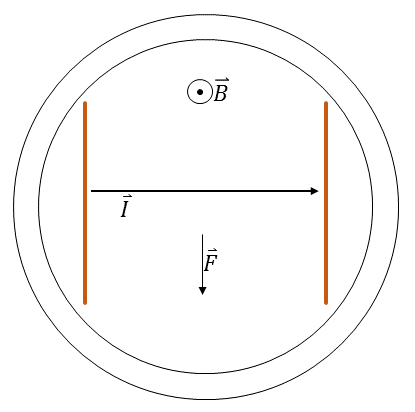
\includegraphics[width=0.5\textwidth]{Oldversion}
	\caption{First iteration of contactless stirrer}
	\label{fig:oldversion}
\end{figure}
Assuming time-invariance, the force applied on a differential element $\mathrm{d}V$ in a current field $\vec{J}$ and an orthogonal magnetic field $\vec{B}$ can be found from the element length d$\ell$ parallel to the current and cross-sectional area d$A$ normal to the current:
\begin{align}
\vec{F}=q\vec{V}\times\vec{B}\\
\vec{F}=I\vec{\ell}\times B\\
I=\lvert J\rvert\mathrm{d}A\\
\end{align}
(Valid because d$A$ is defined to be normal to $\vec{J}$.)
\begin{align}
\mathrm{d}\vec{F}=\lvert\vec{J}\rvert\mathrm{d}A\mathrm{d}\ell\times\vec{B}
\end{align}
Since, in this case, the magnetic and current fields are orthogonal, and since the current field is approximately uniform between the electrodes (simply the total current divided by the electrode area),
\begin{align}
\mathrm{d}\vec{F}=\lvert\vec{J}\rvert\lvert\vec{B}\rvert\mathrm{d}A\,\mathrm{d}\ell\\
\vec{F}=\iiint\limits_V\lvert\vec{J}\rvert\lvert\vec{B}\rvert\mathrm{d}A\,\mathrm{d}\ell
\end{align}
Given an electrode area of $A$ and spacing of $L$ and approximating both the current and magnetic field to be uniform between the electrodes,
\begin{align}
\vec{F}=\lvert\vec{B}\rvert L\iiint\limits_A\lvert\vec{J}\rvert\mathrm{d}A=\lvert\vec{B}\rvert IL
\end{align}
\par This design did work in principle; the Lorentz force produced a pumping action, where fluid would flow down the centerline between the electrodes and recirculate along the walls of the tumbler. However, since a large current was flowing through a fluid, significant electrolysis occurred, which, in addition to producing potentially dangerous hydrogen and oxygen gas, affected the taste of the cocktail due to the electrolysis products.

\section{Theoretical Background}
\par Since the basic application of Lorentz force to pumping was effectively validated (and is in fact well studied \cite{yamato}), the major problem remaining was the electrolysis of the cocktail. As per Faraday's Law of Electrolysis:
\begin{equation}
\dot{m}=\frac{I}{F}\frac{M}{z}
\end{equation}
Where:
\begin{itemize}
	\item $\dot{m}$ is the mass of electrolysis products appearing at an electrode per unit time;
	\item $I$ is the total current flowing into or out of the electrode;
	\item $F$ is the Faraday constant, 96485 mol/C;
	\item $M$ is molar mass of the original substance;
	\item $z$ is the number of valence electrons of the substance.
\end{itemize}
\par Since $F$ is a constant and $M$ and $z$ are properties of the substance, in order to minimize $\dot{m}$, $I$ must be minimized. However, pumping force is also directly proportional to $I$. The central proposal of this project is that currents which circulate entirely within a fluid will not result in electrolysis, because the \textit{net} current flow through the fluid is zero. 
\par The obvious question is how to produce currents without an external EMF source such as a battery. The proposed solution is to use an external, time-variant magnetic field to induce circulating currents (eddy currents) in a conductive fluid.

\par For the purposes of a first-pass analysis, the following model will be considered:
\begin{itemize}
	\item The fluid will be a 3'' diameter, 3'' tall cylinder (based on an approximate cocktail tumbler);
	\item The fluid will be considered to have electrical resistivity $\rho$ and magnetic properties equal to a vacuum (water is in fact weakly diamagnetic, but this is expected to be a negligible contribution);
\end{itemize}

\par Since, at this point, the goal is to find the form of the current field and its dependence on $B_{s,max}$ and $\rho$, it is not necessary to accurately know the resistivity of an actual cocktail; those values are calculated separately.

\par In fact, this application is an adaption of the well-studied eddy current brake (Fig. \ref{fig:eddy_current_brake}).
\begin{figure}[h!]
	\centering
	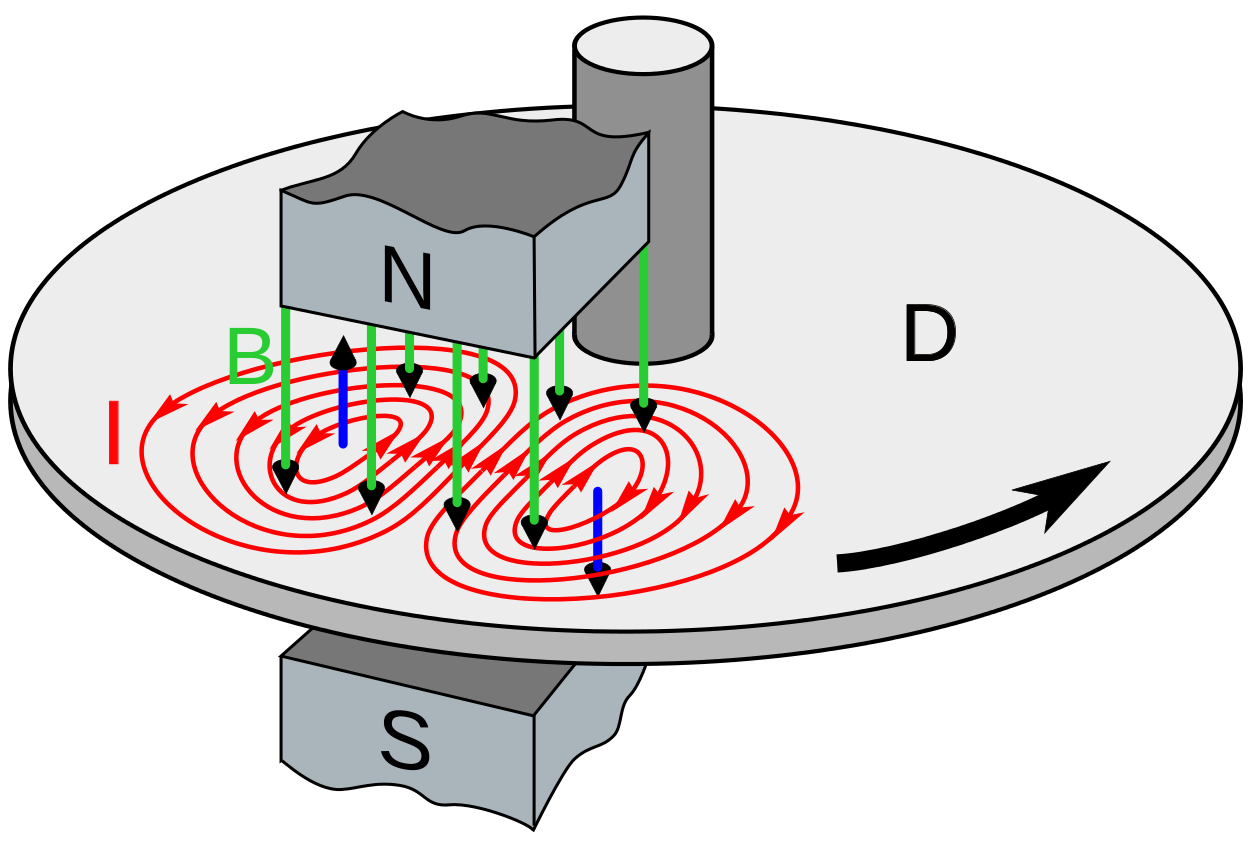
\includegraphics[width=0.5\textwidth]{Eddy_current_brake_diagram}
	\caption{Eddy current disk brake}
	\label{fig:eddy_current_brake}
\end{figure}
In this case, however, the magnets are made to spin, resulting in ``dragging'' of the cylinder. Specifically, if a magnetic field passing through a conductive cylinder radially is made to rotate about the cylinder's axis, currents will be produced in the cylinder, which interact with the field via Lorentz force. Since the strength of the eddy currents, and by extension the resulting force, is proportional to $\frac{\mathrm{d}B}{\mathrm{d}t}$, both the strength of the applied magnetic field and its rate of change should be maximized. 
\subsection{General Design}
\par The obvious way to produce a strong time-variant magnetic field is with an AC solenoid: they are well characterized and fairly easy to control, and of course relatively easy to build. Unfortunately, to produce the high field strengths needed (on the order of 1 T), the power required for a normal solenoid exceeds the capabilities of household circuits. Due to the expense and safety issues, a superconducting solenoid was not practical. Therefore, large permanent magnets were considered. 3'' dia. x 1'' thick NdFeB45 magnets from United Nuclear Scientific LLC were chosen based on field strength per dollar (\$140 and maximum $\vec{B}\cdot\vec{n}$ of $\approx$0.42 T). In order to produce the greatest possible magnetic field, four of these magnets are arranged in a quadrupole configuration. In addition, high-permeability material (in this case, 1020 steel) is used to provide return paths for the field, further increasing the intensity inside the assembly (Fig. \ref{fig:field_in_cup}).
\begin{figure}[h!]
	\centering
	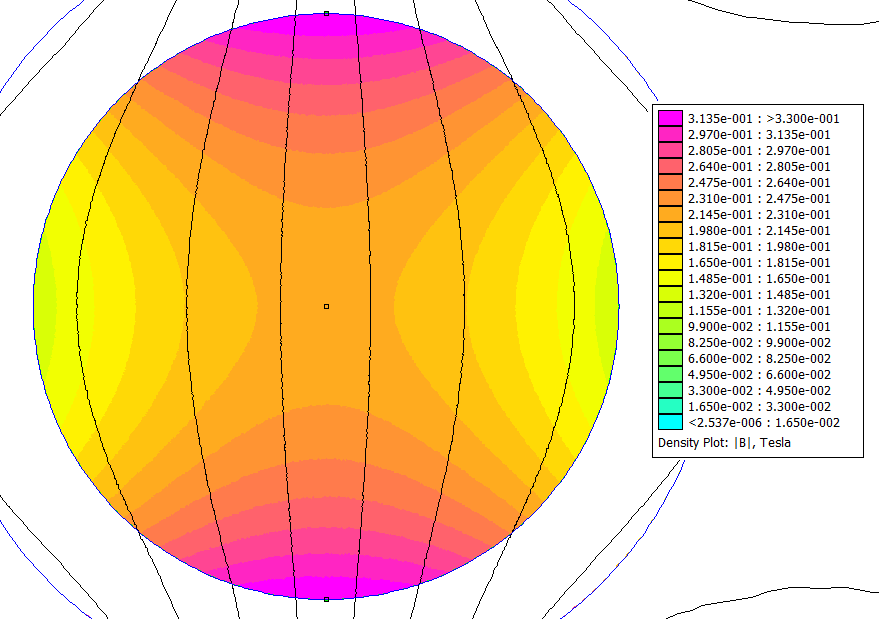
\includegraphics[width=0.75\textwidth]{FieldInCup}
	\caption{Quadrupole magnet assembly with steel shunts}
	\label{fig:field_in_cup}
\end{figure}
\par The downside of permanent magnets, of course, is that they must be in motion to produce a time-variant field. In this case, the quadrupole assembly must be spun about the axis of the cocktail, producing circular forces on the liquid (Fig. \ref{fig:volume_force_density}).
\begin{figure}[h!]
	\centering
	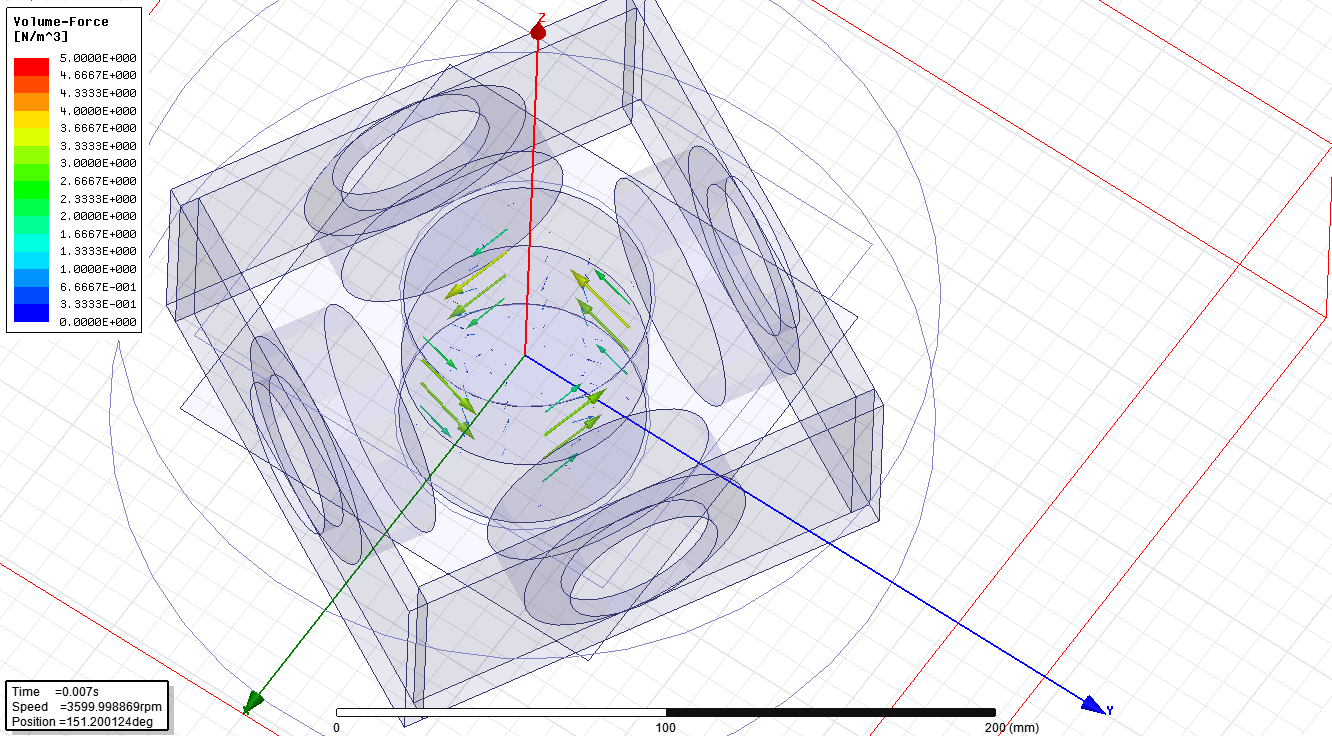
\includegraphics[width=0.75\textwidth]{VolumeForceDensityStill}
	\caption{Volume force density caused by counterclockwise spinning quadrupole}
	\label{fig:volume_force_density}
\end{figure}

\section{Rotor Design}

\section{Property Measurements}
\subsection{Cocktail Resistivity}
\label{sec:resistivity}
\subsection{Rotor Field Measurement}



\begin{thebibliography}{3}
	\bibitem{yamato}
	Takezawa, Setsuo et al. ``Operation of the Thruster for Superconducting Electromagnetohydrodynamic Propulsion Ship YAMATO 1.'' Bulletin of the M.E.S.J 23.1 (1993): 46-55. Japan Institute of Marine Engineering. Web. 21 Aug. 2016. \textless http://www.jime.jp/e/publication/bulletin/english/pdf/mv23n011995p46.pdf>.\textgreater
	
	\bibitem{curesistivity}
	Matula, R. A. ``Electrical Resistivity of Copper, Gold, Palladium, and Silver.'' \textit{Journal of Physical and Chemical Reference Data} 8.4 (1979): 1161. Web. 23 Aug. 2016. \textless http://www.nist.gov/data/PDFfiles/jpcrd155.pdf\textgreater. 
	
	\bibitem{analyticeddy}
	Bowler, John R., and Theodoros P. Theodoulidis. ``Eddy Currents Induced in a Conducting Rod of Finite Length by a Coaxial Encircling Coil.'' Journal of Physics D: Applied Physics 38.16 (2005): 2861-868. Web. 23 Aug. 2016. 
\end{thebibliography}
\end{document}
